\subsection{FDM vs.\ FEM Discretization}

Figure \ref{fig:discretization-comparison} compares the finite‑difference (FDM) and finite‑element (FEM, FEniCSx) discretizations when both are supplied with their analytical Jacobians. The test runs at a fixed grid size \(N_x = 5000\), tolerance \(10^{-10}\), and \(\varepsilon = 10^{-10}\), sweeping the nonlinearity index \(p = 3\) to \(6\) for LSODA and CVODE.

FDM is consistently faster. At \(p = 4\), LSODA completes in 24.4s with FDM but needs 37.4s with FEM – a 53\% overhead. CVODE exhibits a similar pattern: 14.0 seconds (FDM) versus 21.7 seconds (FEM) at the same \(p\). This gap persists across the entire \(p\) sweep, with FEM execution times roughly 1.5–2× those of FDM for both solvers. The primary source of the overhead is the underlying assembly process required by the weak (variational) formulation. FDM bypasses these steps entirely by computing algebraic stencil expressions directly on a structured grid.

However, the FEM path offers a critical advantage in practice. The analytical Jacobian is trivially obtained from the UFL definition of the residual and incurs no manual derivation. Moreover, the FEniCSx implementation generalises to higher spatial dimensions without changes to the solver infrastructure, whereas the finite‑difference stencils would have to be completely re‑derived. For one‑dimensional benchmarks, FDM is the clear winner, but for simulations in 2D or 3D, the greater geometrical flexibility offered by FEM is paramount.

\begin{figure}[H]
  \centering
  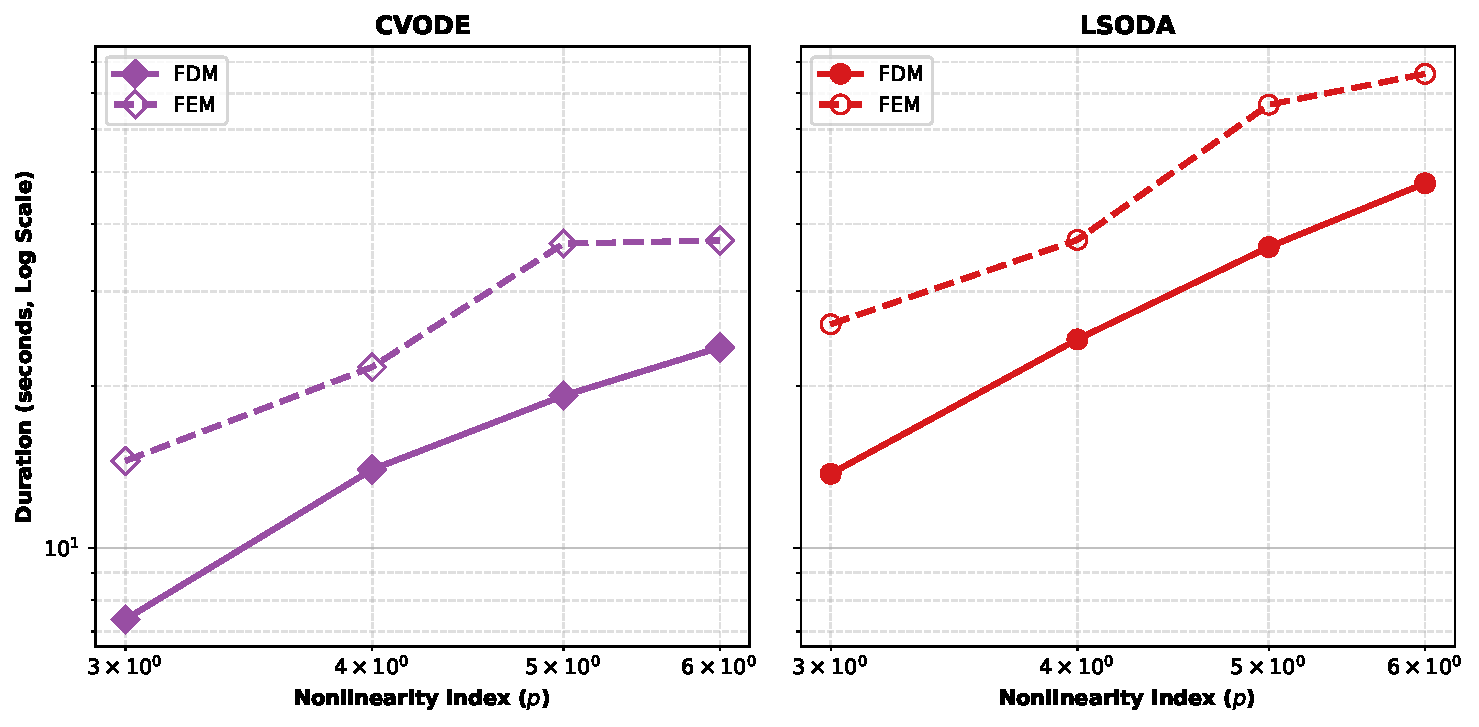
\includegraphics[width=\textwidth]{images/discretization_comparison.pdf}
  \caption{Execution time scaling of analytical‑Jacobian runs for FDM vs.\ FEM discretizations (\(N_x = 5000\), \(\varepsilon = 10^{-10}\), tolerance \(10^{-10}\)).}
  \label{fig:discretization-comparison}
\end{figure}
